\subsection{A complete learned reserve model with an execution decision}\label{sec:complete-model}
This experiment connects hidden inventory, survival-aware filtering, a learned intensity map, exact sampling, and execution evaluation in one model. All rate specifications and labels are synthetic. The model has one displayed ask lot $D=1$, hidden reserve $H\in\{0,\ldots,5\}$, and a fixed hidden regime $R\in\{0,1\}$. Initially $\mathbb P(R=1)=0.4$ and independently $H$ equals $0,2,5$ with probabilities $0.1,0.5,0.4$. This is an explicitly specified aggregate reserve model, not a claim about an exchange's priority rules.

While the trader's passive order is active, the rates are
\begin{equation}\label{eq:complete-rates}
 \lambda_{R,H}=(1+2R)(1+0.08H),\qquad
 \phi_{R,a}=(0.6+0.5a)(0.8+0.4R),\quad a\in\{0,1\}.
\end{equation}
A competing execution consumes the displayed lot. When $H>0$, its mark records a one-lot refresh and updates $(D,H)$ to $(1,H-1)$. When $H=0$, its mark records depletion and the episode ends. An independent passive-fill clock of rate $\phi_{R,a}$ ends the episode with a trader fill. Thus every execution-linked update obeys \eqref{eq:reserve-conservation}. The fill opportunity and its action response are specified parts of this toy market, not inferred counterfactual effects.

The three marks are refresh, depletion, and trader fill. Give each mark a unit-mass event cell; then the conditional rate field is the three-vector
\[
 f(R,H,a)=(\lambda_{R,H}\mathbf1_{\{H>0\}},
          \lambda_{R,H}\mathbf1_{\{H=0\}},\phi_{R,a}),\qquad M=3.
\]
Embed the twelve active hidden states as distinct unit basis vectors in $\R^{12}$. Distinct states are at distance $\sqrt2$. This finite latent geometry accommodates the inventory feasibility indicator directly; no continuous sensitivity is inherited through a discontinuous rounding map.

\paragraph{What is trained.}
A $3$--$24$--$24$--$2$ network with tanh hidden layers and output $10\operatorname{sigmoid}$ receives $(2R-1,H/2.5-1,2a-1)$ and predicts $(\lambda,\phi)$. It has 746 parameters. Training uses all 24 active state/action specifications, with 1,200 Adam updates followed by L-BFGS. The labels are the exact rates in \eqref{eq:complete-rates}; the model is a learned rate emulator, not a market-data estimator. Its finite-domain audit covers every deployed input. This choice isolates whether a learned representation can be inserted into the full probabilistic construction without leaving unmeasured approximation error.

The final mean squared rate error is $4.9514\times10^{-7}$. Exhaustive evaluation gives
\begin{align}\label{eq:complete-constants}
 \epsilon_\lambda&=\max_{R,H,a}\sum_e|f_e-\widehat f_e|=0.00266924,\\
 r_{\max}&=\max_{R,H,a}\|f-\widehat f\|_2=0.00190530,
 \qquad K=3.64972.\notag
\end{align}
Here $K$ is the maximum pairwise learned field difference divided by $\sqrt2$ over required latent states and actions. Both models have total rate below six. The common thinning envelope is therefore $c=6$ on this fully enumerated domain. The analytic bounds are exact mathematical implications; their reported numerical evaluations use float64 and are not interval-arithmetic proofs.

\paragraph{The filter and the decision.}
Before the trader posts, there is no trader-fill clock. For an observed prehistory, the posterior is updated by \eqref{eq:survival-filter}, followed at every refresh by the corresponding likelihood and reserve decrement. We compare three information states: the initial prior; a quiet interval of length $0.5$; and refreshes at $0.1$ and $0.3$ followed by observation through $0.5$. These are specified conditioning histories with positive likelihood density, not selected realized trading records. The neural model uses its own rates to compute its posterior on the same history.

After the two refreshes, the true posterior mean reserve is $1.417759$ and the fast-regime probability is $0.648446$. Dropping survival information gives posterior TV error $0.208696$. The correctly updated neural posterior has TV error $7.97\times10^{-5}$. A direct likelihood calculation over initial states verifies the recursive filter to $5.6\times10^{-17}$.

The trader selects an action $a\in\{0,1\}$ and deadline $\tau\in\{0,0.1,\ldots,1.5\}$. A passive fill costs $0.04a$, depletion before fill costs $1$, and crossing at the deadline while still active costs $0.3$. Costs are per lot in a declared currency unit, with $B=1$. The finite class has 32 configurations and is optimized by enumerating their expected costs. It is a deadline policy class, not the unrestricted solution of a partially observed control problem.

The full model is a 14-state CTMC: twelve active hidden states and two absorbing outcomes. If $p$ is the posterior at the decision origin, $p^Te^{\tau Q_a}$ gives its exact outcome probabilities up to matrix-exponential numerical precision. A neural posterior $\widehat p$ and generator $\widehat Q_a$ give the corresponding model values. No path Monte Carlo is used to choose or value these policies.

\begin{table}[htbp]
\centering\small
\begin{tabular}{lrrrrr}
\toprule
History & Action & Deadline & True cost & Max. value error & Path bound \\
\midrule
initial & 1 & 1.5 & 0.244577 & 1.75e-05 & 4.00e-03 \\
quiet & 1 & 1.5 & 0.223617 & 2.99e-05 & 4.06e-03 \\
two refreshes & 0 & 0.0 & 0.300000 & 7.50e-05 & 4.08e-03 \\
\bottomrule
\end{tabular}

\caption{Exact finite-state policy evaluation. The maximum value error is over all 32 policies at the stated history. The final column is a uniform full-path certificate for the entire deadline class; it is not measured path TV.}\label{tab:complete-model}
\end{table}

Write $\delta_0=\TV(p,\widehat p)$. Couple these initial hidden states maximally and then apply common-event thinning. For every policy in the class,
\begin{equation}\label{eq:complete-path}
 \TV(P^a,\widehat P^a)\le
 1-(1-\delta_0)e^{-1.5\epsilon_\lambda}.
\end{equation}
This gives the final column of \Cref{tab:complete-model}. The same argument bounds the joint hidden-state/history laws at each earlier time, so \Cref{prop:filter-stability} and the $W_1$ version of \Cref{lem:posterior} also give the separate field/posterior certificate
\begin{equation}\label{eq:complete-field}
 \sqrt3\left[1.5r_{\max}
 +2\sqrt2K\int_0^{1.5}\{1-(1-\delta_0)e^{-\epsilon_\lambda t}\}\dd t\right].
\end{equation}
Its values are $0.05857$, $0.06021$, and $0.06070$. The direct full-state coupling is substantially tighter in this small enumerated model. Reporting both shows the price of the representation-level decomposition; it does not conceal it behind the abstract theorem.

The learned and true models select the same policy in each information state, giving zero regret within the enumerated class. After the prior or quiet history, action $1$ with deadline $1.5$ is preferred; after two refreshes, immediate crossing is preferred. The uniform regret bounds are about $0.0080$--$0.0082$ currency units. The corresponding 99-percent CVaR error bounds are $0.3996$--$0.4075$ units, below the trivial bound $B=1$. Several actual policies have CVaR equal to the worst cost; a nontrivial bound is not evidence that their tail losses are small.

\paragraph{Sampling independently checked.}
We implement both exact averaging and one fresh posterior draw per proposal, updating the entire belief after accepted marks. In 20,000 paths for each method, with action $1$, horizon $0.8$, and the two-refresh posterior, all three terminal probabilities agree with matrix exponentiation within five binomial standard errors. Maximum absolute discrepancies are $0.00356$ and $0.00739$. These are sampling diagnostics; exactness of the construction follows from \Cref{prop:posterior-thinning}.

\begin{figure}[htbp]
\centering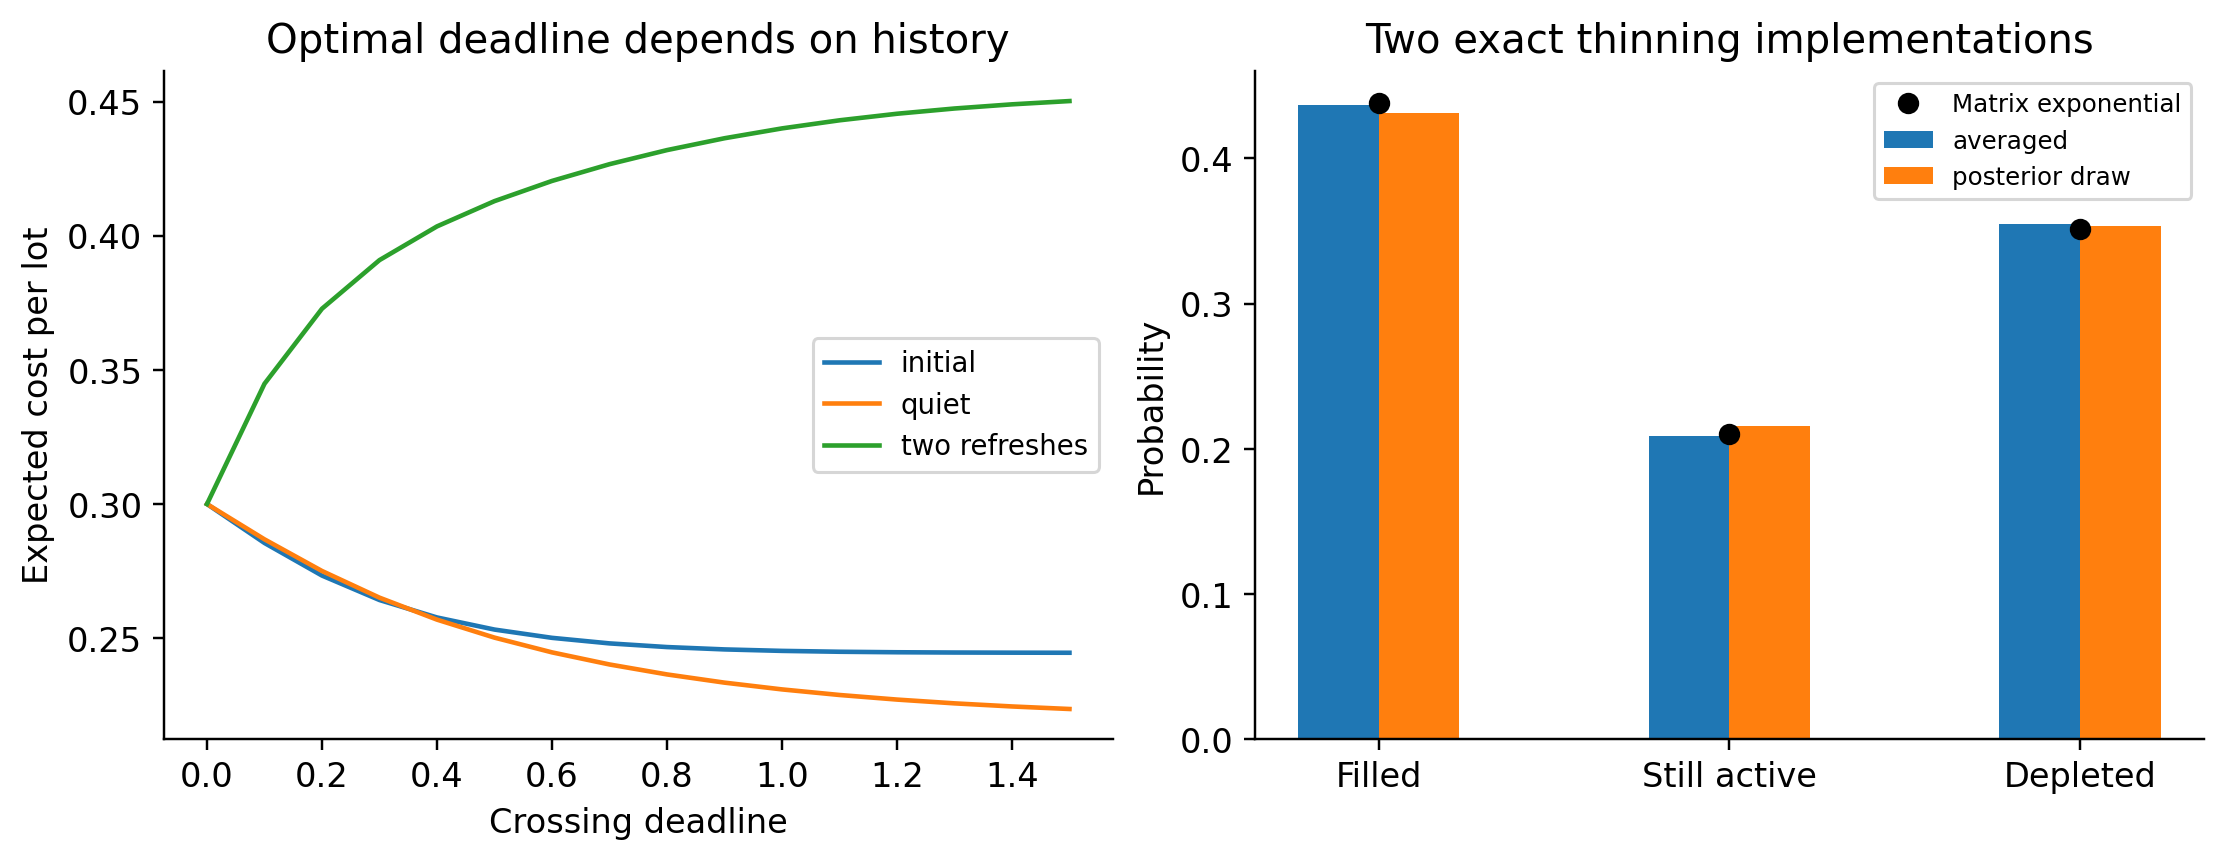
\includegraphics[width=\textwidth]{figures/learned_reserve.png}
\caption{Left: true expected execution cost, minimized over the two action choices at each deadline, for three observed histories. Right: two thinning implementations compared with independently computed CTMC outcome probabilities.}\label{fig:complete-model}
\end{figure}

\subsection{A genuinely adapted volatility perturbation}
To test \Cref{thm:vol-price}, use 32 equal steps over $T=1$ and let
\[
 W_n=\sum_{k<n}\sqrt{\Delta_k}Z_{k+1},\qquad
 \sigma_n=0.2+0.1\tanh(W_n),\qquad
 \widehat\sigma_n=\sigma_n+\delta.
\]
Both volatilities are selected before the next return innovation. For
$\delta\in\{0.005,0.01,0.02\}$, take the common bound $\bar\sigma=0.32$.
The theorem input is exactly $\mathcal A_N=\delta^2$, not an estimated future-path transport distance. From 200,000 common-innovation paths with $X_0=100$, the at-the-money call differences are $0.199253$, $0.398629$, and $0.797714$, with standard errors $0.000892$, $0.001789$, and $0.003602$. The improved deterministic bounds are $0.694672$, $1.389344$, and $2.778688$. Estimated absolute terminal coupling errors are $0.400444$, $0.800891$, and $1.601781$. The bound controls these coupled constructions and Lipschitz payoffs; it is not an assertion that this coupling realizes $W_1$.
